\documentclass[11pt]{article}

\pdfminorversion=4

% use packages
\usepackage[utf8]{inputenc}
\usepackage{amsmath}
\usepackage{amsthm}
\usepackage{amsfonts}
\usepackage{amscd}
\usepackage{amssymb}
\usepackage{natbib}
\usepackage{url}
\usepackage[table,xcdraw,usenames]{xcolor}
%\usepackage[usenames]{color}

% \usepackage[pdftex,active,tightpage]{preview}
% \setlength\PreviewBorder{2mm}

\usepackage{tikz}

% \usetikzlibrary{arrows,positioning, calc}
% \tikzstyle{vertex}=[draw,fill=black!15,circle,minimum size=20pt,inner sep=0pt]

\usetikzlibrary{trees}

% \usepackage{tikz-qtree,showframe}

\usepackage{forest}


\usepackage{graphicx}
\usepackage{subcaption}
\usepackage{mathtools}
\usepackage{enumitem}
\usepackage{authblk}
\usepackage{bm}
\usepackage{comment}
\usepackage{pdfpages}

\usepackage{hyperref}
\usepackage{caption}
\usepackage{float}
%\usepackage[caption = false]{subfig}
\usepackage{tikz}
\usepackage{multirow}
\usepackage[linesnumbered, ruled,vlined]{algorithm2e}
\usepackage{pdflscape}
\usepackage{etoolbox}

%\AtBeginEnvironment{align}{\setcounter{equation}{0}} % https://tex.stackexchange.com/questions/349247/how-do-i-reset-the-counter-in-align

% margin setup
\usepackage{geometry}
\geometry{margin=0.8in}

% function definition
\newcommand{\V}{\textbf{V}}
\newcommand{\weight}{\pi}
\newcommand{\ret}{\textbf{r}}
\newcommand{\y}{\textbf{y}}
\newcommand{\w}{\textbf{w}}
\newcommand{\x}{\textbf{x}}
\newcommand{\dbf}{\textbf{d}}
\newcommand{\X}{\textbf{X}}
\newcommand{\Y}{\textbf{Y}}
%\newcommand{\L}{\textbf{L}}
\newcommand{\Hist}{\mathcal{H}}
\newcommand{\Prob}{\mathbb{P}}
\def\mbf#1{\mathbf{#1}} % bold but not italic
\def\ind#1{\mathrm{1}(#1)} % indicator function
\newcommand{\simiid}{\stackrel{iid}{\sim}} %[] IID 
\def\where{\text{ where }} % where
\newcommand{\indep}{\perp \!\!\! \perp } % independent symbols
\def\cov#1#2{\mathrm{Cov}(#1, #2)} % covariance 
\def\mrm#1{\mathrm{#1}} % remove math
\newcommand{\reals}{\mathbb{R}} % Real number symbol
\def\t#1{\tilde{#1}} % tilde
\def\normal#1#2{\mathcal{N}(#1,#2)} % normal
\def\mbi#1{\boldsymbol{#1}} % Bold and italic (math bold italic)
\def\v#1{\mbi{#1}} % Vector notation
\def\mc#1{\mathcal{#1}} % mathical
\DeclareMathOperator*{\argmax}{arg\,max} % arg max
\DeclareMathOperator*{\argmin}{arg\,min} % arg min
\def\E{\mathbb{E}} % Expectation symbol
\def\mc#1{\mathcal{#1}}
\def\var#1{\mathrm{Var}(#1)} % Variance symbol
\def\checkmark{\tikz\fill[scale=0.4](0,.35) -- (.25,0) -- (1,.7) -- (.25,.15) -- cycle;} % checkmark
\newcommand\red[1]{{\color{red}#1}}
\def\bs#1{\boldsymbol{#1}}
\def\P{\mathbb{P}}
\def\var{\mathbf{Var}}
\def\naturals{\mathbb{N}}
\def\cp{\overset{p}{\to}}
\def\clt{\overset{\mathcal{L}^2}{\to}}

\setcounter{tocdepth}{4}
\setcounter{secnumdepth}{4}

\newtheorem{corollary}{Corollary}
\newcommand{\ceil}[1]{\lceil #1 \rceil}
\newcommand{\norm}[1]{\left\lVert#1\right\rVert} % A norm with 1 argument
\DeclareMathOperator{\Var}{Var} % Variance symbol

\newtheorem{cor}{Corollary}
\newtheorem{lem}{Lemma}
\newtheorem{thm}{Theorem}
\newtheorem{defn}{Definition}
\newtheorem{prop}{Proposition}
\theoremstyle{definition}
\newtheorem{remark}{Remark}
\hypersetup{
  linkcolor  = blue,
  citecolor  = blue,
  urlcolor   = blue,
  colorlinks = true,
} % color setup

% proof to proposition 
\newenvironment{proof-of-proposition}[1][{}]{\noindent{\bf
    Proof of Proposition {#1}}
  \hspace*{.5em}}{\qed\bigskip\\}
% general proof of corollary
  \newenvironment{proof-of-corollary}[1][{}]{\noindent{\bf
    Proof of Corollary {#1}}
  \hspace*{.5em}}{\qed\bigskip\\}
% general proof of lemma
  \newenvironment{proof-of-lemma}[1][{}]{\noindent{\bf
    Proof of Lemma {#1}}
  \hspace*{.5em}}{\qed\bigskip\\}

\allowdisplaybreaks

\title{Forecast Adjustment Under Shocks: A Unification}
\author{David P. Lundquist\thanks{davidl11@ilinois.edu}, Daniel J. Eck\thanks{dje13@illinois.edu} }
\affil{Department of Statistics, University of Illinois at Urbana-Champaign}
\date{\today}

\begin{document}

\maketitle

\begin{abstract} 
  When should one's default forecasting model be adjusted, augmented, or abandoned completely?  Should it be done algorithmically or via human discretion, and if the latter, where and how should discretion play a role?  Should an adjustment be carried out using external information, and what exactly should be adjusted?  This work further systematizes and unifies the rich landscape of model adjustment and model correction methods, with a special focus on forecast adjustment under the presence of news shocks, when unanticipated events may give an observer reason to doubt the credibility of the default forecasting function.  We demonstrate the usefulness of similarity-based methods in forecasting and present a general framework dubbed Similarity-based Parameter Correction (SPC).  We highlight several specific time series models that can benefit from SPC, along with formal results for some of those special cases.
\end{abstract}


\section{Introduction}\label{Introduction}

In time series and panel data, sometimes the salient challenge is not predicting when an event will occur or begin but what its key properties will be.  In the familiar case of scalar time series, those properties can include the time series' post-event direction, magnitude of change, moments, duration of the event, or correlation structure, all over an arbitrary horizon or perhaps multiple horizons. This is not to say that predicting the arrival of an event is easy. In some cases, it may be difficult or impossible.  The event might not even be conceivable to many before it happens, as was the case with the COVID-19 pandemic.  There, reacting sensibly to a shock or structural change may best one can hope for.  On the other end of the spectrum are events whose arrival need not be predicted because they are scheduled in advance, e.g. scheduled news, like releases of economic data or election results.  In those cases, conditional forecasts allow a statistician to proceed as if the event has arrived.  Consider the analysis of Mike Wilson, Morgan Stanley’s CIO and Chief US Equity  Strategist, in October 2024 regarding the upcoming 2024 US Presidential US \citep{thoughts_on_market}:

\begin{quote}While some argue a Trump win would be a headwind for growth and equity markets, due to tariff  risks and slowing immigration, we think there's an additional element from the 2016 experience that  is worth considering—rising animal spirits. More specifically, in 2016 Trump's pro-business approach  led to the largest 3-month positive impact on small business confidence in the past 40 years. It also translated into a spike in individual investor sentiment. It appears to me that markets may be trying  to front-run a repeat of this outcome as Trump's win in 2016 came as a surprise to pundits and  markets alike.
\end{quote}
Wilson here assesses how market participants are incorporating current information as well as information about past forecast failures, including the potential overweighting of more recent failures.  His assessment implies that the shock conditional on a Trump victory may disappoint observers, as it has already been pulled forward into current forecasts.  In short, this time around may be different.  What Wilson is engaging in is what \cite{lundquist2024volatility} identify as a crucial reaction to  events: what, if anything, does it resemble from the past?

Herein we attempt to unify a range of conceptual approaches to forecasting amid shocks that have developed across the broad ecosystem of the econometric and forecasting literatures.  We attempt to locate our main contribution, Similarity-based Parameter Correction, at the intersection of several important strands of thought.  We in fact delineate a specific type of SPC called post-shock forecasting, which is induced by nuanced and interesting choices that fall under the general SPC framework.  In particular, this work focuses on model adjustment amid news shocks that undermine the reliability of the  model at hand.  Forecasting under shocks raises unavoidable questions: should the forecast model be abandoned in favor of a discretionary or ad-hoc or one-off adjustment?  Does the does the discretion of a forecaster rule out a quantitative method for making the adjustment?  What is the ultimate purpose of the adjustment, and how it is to be used?  For how long is the adjustment necessary or reliable?

Forecast model adjustment received its earliest attention under the auspices of ``intercept correction" \citep{hendry1994theory,clements1996intercept,clements1998forecasting, clements1999forecasting}.  Of fundamental importance is the distinction between discretionary and automated intercepts corrections. \cite{hendry1994theory} define scalar intercept corrections to be automated when they follow the simple rule of adding an estimation or prediction residual $e_{t}$ to subsequent (possibly but not necessarily all) forecasts $\hat f_{t+1},\hat f_{t+2},[...].$ ``\textit{[S]etting the model back on track}" is the informal label they provide for that procedure.  It must be noted here that adding a past residual to future forecasts assumes implicitly that whatever caused the residual has some persistence.  Hence, intercept correction might be thought more appropriate for time series of levels, or at least times series of rates that are not necessarily mean-reverting, like inflation.  Of course, if one has a strong grasp of how long the intercept correction will be necessary, then all of that is moot, but in practice, knowledge of that persistence may be harder to come by than foreknowledge of the need for intercept correction. 
 
The term intercept correction can be construed more broadly to encompass correction of terms besides the intercept, and justification for it can be found beyond the original goal of setting forecasts back on track.  In later work, \cite{clements1999forecasting} add seven additional interpretations for intercept correction, and \cite{hendry1994theory, clements1999forecasting} themselves note the possibility of correcting a coefficient in a forecast model specification, and \cite{guerron2017macroeconomic} developed a similarity-based procedure for correcting the parameter $\beta$ using past information of the time series itself.   For a review of more recent work in similarity-based forecasting, we refer the reader to \cite{lundquist2024volatility}.

What if the break in the DGP is brought about by a very particular kind of event, a news shock?   What if we could predict well the intercept shift that occurs between $T^{*}$ and $T^{*}+1$?  In \cite{castle2016overview}, the authors list six necessary conditions for reacting to what we in this current paper call a news shock.  Of greatest interest to us are two of the six: 

\begin{itemize}
\item ``the forecasting model already embodies that source of information" and 
\item ``there is an operational method for selecting an appropriate model".
\end{itemize}   

For intercept shifts that occurs between $T^{*}$ and $T^{*}+1$, forecasting procedures have been explored in \cite{lin2021minimizing,lundquist2024volatility}, where the AR(1) and GARCH($m,s$) cases, respectively, are treated.  Both works target additive parameters in scalar time series, predicting the additive parameter in the time series under study by aggregating information from other time series.  The authors leave several stones unturned, including a more general, dare say comprehensive treatment of how to forecast under any sort of shock.

As the literature has developed, a current practitioner of forecast adjustment can now choose between (i) procedures that are discretionary or automated, (ii) adjusting using internal data (i.e. from the time series itself) or external, (iii) the term to be corrected (e.g. intercept, coefficients), if any, (iv) as well as the specification of the correction function (i.e. the mapping from the donor unit data to the correction term in the time series under study), including the aggregation mechanism applied to the assembled data (e.g. Nearest-Neighbor, arithmetic mean, kernel methods).  We discuss this in depth in Section \ref{global_overview}.

If intercept correction is the correction of a forecast by adding the residual at time $T^{*}+1$ to the forecasts at some subset of $\{T^{*}+2,T^{*}+3,...\}$, in this manuscript, we are doing something rather close to that by adding the predicted correction term to each forecast in some some subset of $\{T_{1}^{*}+1,T_{1}^{*}+2,...\}$, where $T^{*}_{1}+1$ is first integer index for the time series under study following the shock. 
The general procedure presented, post-shock forecasting, is a discretionary procedure for intercept correction that integrates data internal or external to the time series under study in a systematic manner.  It is a discretionary procedure in the sense that substantive choices must be made at each instance of use.  The correction function uses the notion of similarity at multiple levels: first, to identify similarity between breaks in different time series, and second, in borrowing from the causal inference literature to aggregate information from those similar circumstances.  Parametric specifications for location shifts in the DGP can be found in \cite{castle2011forecasting}, where locations shifts are modeled as induced by additional observable variables, as well as in \cite{lundquist2024volatility}, where the arrival of the news shock is observable, even if its quantitative instantiation is not.  Beyond \cite{lin2021minimizing,lundquist2024volatility}, we are not aware of prior work that proposes a method for aggregating similar shocks occurring outside the time series under study in order to correct the time series under study.


The structure of this manuscript is as follows.  We provide a deeper and more critical review of several literatures, including intercept correction, model-evaluation, and similarity-based forecasting.  We then provide a canonical setting in which we attempt to focus our work.  This setting will be presented at a level of generality that showcases the broad applicability of our method.  We then introduce the method from a global perspective, abstracting away from familiar applications.  We then show several specific applications, including novel applications that cannot be found elsewhere in the literature.  We close with a discussion, including possible extensions.

 \section{Forecasting Amid Shocks}

% \begin{preview}
% \begin{tikzpicture}[very thick,level/.style={sibling distance=180 mm/#1}]
% \node [vertex] (r){Forecast Model Adjustment}
%   child {
%     node [vertex] (a) {Break in the GDP at $T^{*}$}
%     child {
%       node [vertex] {$20$}
%       child {
%         node [vertex] {$-3$}
%         child {node [vertex] {$17$}}
%         child {node [vertex] {$5$}}
%       }
%       child {node [vertex] {$6$}}
%     }
%     child {
%       node [vertex] {$3$}
%       child {node [vertex] {$7$}}
%       child {node [vertex] {$2$}}
%     }
%   }
%   child {
%     node [vertex] {Break in the GDP at $T^{*}$}
%     child {
%       node [vertex] {$8$}
%       child {node [vertex] {$2$}}
%     }
%     child {
%       node [vertex] {$11$}
%       child {node [vertex] {$17$}}
%       child {node [vertex] {$-4$}}
%     }
%   };
% \end{tikzpicture}
% \end{preview}


% https://tex.stackexchange.com/questions/64148/tikz-label-on-tree-edge

% \begin{forest}
% for tree={circle,draw, l sep=20pt}
% [3,red 
%     [1  
%       [4,edge label={node[midway,left] {Help!}} ] 
%       [1] 
%       [3]
%     ]
%     [2
%       [3] 
%       [2] 
%       [5]
%   ] 
% ]
% \end{forest}


%https://tex.stackexchange.com/questions/64148/tikz-label-on-tree-edge

%  \begin{tikzpicture}[level distance=1.5cm,
%   level 1/.style={sibling distance=3.5cm},
%   level 2/.style={sibling distance=2.5cm}]
%   \tikzstyle{every node}=[circle,draw]
  
% \node (Root) [red] {Is there a break in the DGP between T* and T*+1?} 
%     child {  edge from parent node[left,draw=none] {Do you have information outside of the “regular forces”
%     } 
%     node {Yes} 
%     child { node {Yes} 
%             child { node{Yes} edge from parent node[left,draw=none] {lab} }
%             child { node{No}}}
%     child { node {No} }
% }
% child { 
%     node {No}
%     child { node {Yes} }
%     child { node {No} }
% };
% \end{tikzpicture}

% \noindent\begin{forest}
%   for tree={
%     parent anchor=south,
%     child anchor=north,
%     edge path={
%       \noexpand\path [\forestoption{edge}] (!u.parent anchor) -- +(0,-5pt) -| (.child anchor)\forestoption{edge label};
%     }
%   }
%   [Is there a break in the DGP between T* and T*+1?
%     [Extractive Summarization
%       [Similarity
%         [Topic]
%         [Cluster]
%       ]
%       [Classification
%         [test2]
%         [test1]
%       ]
%       [Feature Selection
%         [test1]
%         [test2]
%         [test3]
%       ]
%       [Feature Extraction
%         [test2]
%         [test3]
%       ]
%     ]
%     [Abstractive Summarization]
%   ]
% \end{forest}
% \bigskip

% https://tex.stackexchange.com/questions/539600/tikz-forest-coloring-and-edge-label-positions

% \tikzset{eln/.style={midway, font = \scriptsize,circle,inner sep=2pt}}
% \begin{forest}
% for tree = {circle, 
%     draw=red, %<-added =red
%     minimum width = 2.25em,
%     l sep+=2em
% }
%     [\textcolor{blue}{Is there a break in the DGP between T* and T*+1?
% }
%         [Dog, edge label = {node [above left,eln] {\textcolor{green}{Yes}}}
%             [$B$, edge label = {node [above left,eln] {$4$}}
%                 [$D_1$, edge label = {node [left,eln] {$7$}}
%                     [$G_1$, edge label = {node [left,eln] {$10$}}]
%                 ]
%             ]
%             [$C$, edge label = {node [above right,eln] {$2$}},edge=blue%<-blue edge
%                 [$D_2$, edge label = {node [above left,eln] {$3$}}
%                     [$G_2$, edge label = {node [left,eln] {$6$}}]
%                 ]
%                 [$G_3$, edge label = {node [above right,eln] {$4$}}]
%             ]
%         ]
%         [$G_4$, edge label = {node [above right,eln] {\textcolor{red}{No}}}]
%    ]
% \end{forest}

%https://tex.stackexchange.com/questions/226435/reducing-forest-tree-width-without-squashing


%https://tex.stackexchange.com/questions/244006/making-forest-tree-with-lots-of-text-much-narrower
\begin{figure} 
  \centering  
\resizebox{\textwidth}{!}{%
\begin{forest}
  /tikz/every node/.append style={font=\small},
  for tree={
    rounded corners, 
    % top color=gray!5, bottom color=gray!30, 
    edge+={darkgray, line width=4pt}, 
    draw=darkgray, 
    l sep=.8cm,
    s sep=.5cm,
    minimum height=8.8cm,
    minimum width=1cm,
    child anchor=west,
    parent anchor=east,
    grow'=east,
  minimum size=1cm,%new possibility
  text width=4cm,%
    draw,
    anchor=west,
    edge path={
      \noexpand\path[\forestoption{edge}]
        (.child anchor) -| +(-5pt,0) -- +(-5pt,0) |-
        (!u.parent anchor)\forestoption{edge label};
    },
  }
    [Break in the DGP between $T^{*}$ and $T^{*}+1$?,fill=blue!30 
        [Is there information outside of “regular forces” \citep{castle2011forecasting},edge=green, fill=blue!30%,draw=green
            [Can we use the information outside “regular forces” to forecast (as opposed to merely spotting the break)?,edge=green,,fill=blue!30 
                [Do you have a parametric model (with estimable parameters) for how information outside of ``regular forces” will figure at $T^{*}+h$?,edge=green,fill=blue!30 
                  [What other time series are governed by the parametric model?  How can we extract information from them?  Which are most relevant, %most similar?  How do we determine similarity, quant or qual?  Once we know what is similar, how do we use it?
                  ,edge=green,fill=blue!30 
                  ]
                  [The information that helped spot the break can be used to assemble series that have experienced breaks under similar circumstances. Forecast residuals/losses can be aggregated. %basement for model adjustment for the time series under study.  Without a parametric model, your options are limited but not empty.  With appropriate assumptions on the DGP pre-break and post-break, assumptions on the forecast functions and misses, we can still do things like aggregate residuals and bound forecast loss.
                  ,edge=red,fill=gray!30
                  ]
                  ]
                [Use “regular forces” to do the model adjustment for the post-break period.  Examples of this would include refitting one’s data to use Markov-switching models – i.e. using only the series itself.,edge=red,fill=gray!30
                ]
                ]
                [Then forecasting will require at least one post-break data point to be observed.,edge=red,fill=gray!30]
            ]
            [\cite{clements1998forecasting} discuss this.,edge=red,fill=gray!30]
            ]
        ]
    ]
\end{forest}
}\caption{Forecast Model Adjustment: A Decision Tree}\label{fig:tree}
\end{figure}

 %  To be sure, this manuscript will make its contributions largely in this area.  However, before we get there, let's follow others in asking whether we would ever want to intercept-correct an unconditional forecast as opposed to the conditional.  This is what Clements and Hendry call ``Exploiting the information in unconditional forecasts''.  \cite[p. 170-1]{hendry1994theory} recall how unconditional forecasts can have lower forecast variance than conditional forecasts.  There seems to be two different questions that we should distinguish: we forecast would minimize the conditional expectation of MSE, and what forecast would have the lowest variance.

%  Mismeasured data is discussed in \cite[p. 166]{hendry1994theory} as a motivator for intercept correction.  Could similarity-based correction help?  Here is an idea: if we believe that our most recent measurement of the series is noisy, we can disregard the point itself and instead take a convex combination of that point and the \cite{lin2021minimizing}-style prediction based on aggregation.

% Yet another potential motivation springs from the way we evaluate model performance.  In \cite{clements2005evaluating}, the authors discuss six dichotomies regarding forecast evaluation as a way of advising caution about simplistic notions of performance evaluation.  These ideas matter for the current manuscript for at least one reason.  We must entertain the possibility that breaks in the DGP will invalidate the standard forecast evaluation framework under which we had been working.  If, for example, we have a family of models estimated used a Gaussian loss function, and the post-shock residuals are not conditionally Gaussian (e.g. they could be conditionally Cauchy), then why even start with the default forecasting function?  Why not throw it out entirely?  If only the distribution of the innovations changes, then would that even matter for a forecast that is purely concerned with the conditional mean?

 \cite[p. 177]{hendry1994theory} characterize breaks in the DGP (and hence the misspecification of the default forecasting method) is the ``most obvious and best understood rationale'' for intercept correction.  In this section, we wish to locate the task of forecasting amid shocks within the broader literature on forecasting under breaks in the DGP. 


 A terminological note is in order before we proceed.  We use the term ``shock'' as a special case of a break in the DGP, even though, strictly speaking, some shocks will neither result from a break in the DGP nor herald the emergence of a new regime.  The news shocks examined in this manuscript, however, should be considered breaks in the DGP, no matter whether they are transient or permanent.  Additionally, in this work, we will be focused on news shocks that occur strictly between two discrete time points, or information available at a ``fractional lag" \citep{castle2011forecasting}.  This leads to a further terminological point.  Errors are a staple of stochastic modeling and also go by the synonyms ``noise", ``shocks", or ``innovations''.  The meaning of these terms may not differ as much in their mathematical representations in symbol but in how they're interpreted.  Whereas in the psychometric and social-scientific fields, errors may represent unmeasured or latent capacities of a unit, in other fields like the natural sciences, errors may be used to account for variability in the instruments used to collect data.  ``Innovations" or ``shocks", in econometric literature, are generally understood to represent the arrival of previously unknown (but not necessarily uncontemplated) information.  Shocks are called structural when they are can be linked back to some key feature of an scientific (usually economic) theory; otherwise, they are idiosyncratic.  However, there exist other subcategories of shocks that crosscut the distinction just made.  For example, a news shock is a shock in which the information material to the market is delivered via newsmedia and moves markets no earlier than the news release itself.  Shocks can also be permanent or transitory, supply-related or demand-related, and so forth.  The taxonomy is vast.  What matters for this work is the news shocks we posit occur between two discrete time points, so that a practitioner is faced with the question of what action is most advisable for the following time point, given the news shock.

\subsection{The Role of Outside Information}\label{outside_info}

When is more information better?  That is a central question with regard to forecasting.   In \cite{clements2005guest} (cited in \cite{castle2013forecasting}), the authors note that when forecasts fail, it often has to do with location (i.e. intercept shifts).  Therefore, using additional information is not likely to help unless it can address potential location shifts.  We should clarify what we mean by ``additional information".  Do we mean any information not included in the default forecast function?  Could that include something as straightforward as additional lags of the time series being forecast?  Perhaps a more useful distinction to make is that between information internal to the time series being forecast and information external to the time series being forecast.  Of course, the usefulness of this distinction will hinge, in part, on whether we can cleanly partition information into internal and external buckets.  A cross-cutting distinction originates in \cite{castle2011forecasting}, which discusses necessary conditions for forecasting under breaks as well as a taxonomy of information available for doing so.  The authors make a fundamental distinction between ``regular forces'', which includes the typical standbys of economic theory, and information potentially relevant to location shifts.  

We wish now to sharply distinguish between essential and inessential concepts.  For example, whether information is relevant to location shifts or not is a worthy and complex question that depends upon numerous factors, including but not necessarily limited to the DGP.  However, we would prefer to elide that distinction with internality or externality, or whether the information belongs to the traditional sort of information used in econometric modeling, though certain tendencies and general patterns may emerge.  We make clear what is essential in the table below.

\begin{table}[htb]
  \centering % instead of \begin{center}
  \caption{A 2x2 Schema for Forecast Information, With Examples}
  \begin{tabular}{ | m{3em} | m{6cm}| m{8cm} | } 
    \hline
    & Conventional Econometric Models & Outside Conventional Econometric Models\\ 
    \hline
    internal & Lags of the series itself; past shocks & \\
    \hline
    external & Macro variables like interest rates, commodity prices; weather-related variables & Google Trends, high-frequency data like prediction markets; past shocks under similar conditions \\ 
    \hline
  \end{tabular}
\end{table}
 
  \subsection{The Meaning and Use of Similarity}
This manuscript aims to contribute at the intersection of post-break forecasting and similarity-based forecasting.  In particular, we use the former to motivate the latter.  The notion of similarity appears in various statistical contexts, including matching, synthetic control, nearest-neighbor methods, not to mention the massive area of approximation theory.  The uses of similarity are too sprawling to recount here.  Our objective is to make forecast corrections by exploiting information from previous time series that have undergone shocks under similar circumstances.  The first use of the term ``similar'' is an appropriate point to attempt a definition.  As a provisional definition, we say that a break in the DGP of a time series is similar to a break in another if the causes of the breaks share key, material qualities.  Note here that we have not said anything about the time series themselves (their DGPs or moments) being similar, nor the entities that they represent (e.g. the firms, the financial instruments, the governments, etcetera) being similar.  Why that is so will become clear shortly.

It matters where we look for similarity and how we estimate similarity.  Several distinctions are relevant here.  First, quantitative ways of determining similarity naturally tend toward the idea that similarity is reducible to determining what serves as a best approximation.  Those approaches include matching a target object to other objects along one or more variables, where unique matches or exact matches may be likely or may be statistically certain, likely, unlikely, or impossible, subject to the setting.  In metric spaces, the notion of a metric that quantifies nearness is crucial to fundamental concepts of proximity.  This suggests a set of optimization problems such that for any target object $Q$, the search for similarity means a search for an approximator or collections of approximators $A$ s.t. $\delta(Q,A)$ is smallest, where $\delta$ is an appropriate metric.

The notion of approximating a target does not necessarily mean that the target need be similar to the approximator.  This suggests a role for asymmetric distance functions $\delta$ (which are of course not metrics) for exploring differences between donors and weight their contributions accordingly.  Consider an asymmetric Jaccard Index $\delta_{\mathcal{J}}(\cdot,\cdot)$ that maps from any two finite-cardinality sets to the interval $[0,1]$ \citep{garg2015asymmetric}.  Asymmetry also plays an important role in weighting schemes far beyond traditional forecasting, including Transformer mechanisms inside the field of deep learning.  The asymmetry inherent in query, key, and value matrices allow hierarchical relations in language to be represented mathematically \citep[p. 364]{bishop2023deep}.  

So far, we have discussed only binary measures of similarity.  The distance-based weighting scheme found in \cite{lin2021minimizing} and repurposed in \cite{lundquist2024volatility} can be thought of as an $n$-ary similarity measure, where the $n$ weights means little in isolation but can tell a greater story when viewed alongside the approximation they produce.  However, an $n$-ary similarity measure will not always reduce to the task of constructing an approximator to the target using $n$ original objects.  We might instead insist on a notion of similarity such that $n$ objects are said to be similar, as a collection, to the target if and only if each of the $n$ matches the target perfectly.

What about qualitative ways of determining similarity?  In \cite{lin2021minimizing, lundquist2024volatility}, donors are identified by matching the qualitative aspects of the shock in the time series under study to shocks previously witnessed in other series.  Only after the donor pool has been identified based on qualitative facts about the shocks is there a role for quantitative methods.  The role of the covariate vector in their models is two-fold: the covariates appear in the shock distribution, and the covariates also help determine which donors are most important.  

We pose two questions.  What if a given entry of the covariate vector was helpful at only one of those roles?  For example, what if an entry was particularly useful in yielding good weights but was not important for the shock distribution --- perhaps because the corresponding shock parameter was zero.  

Conversely, suppose a given entry was known to be part of the shock distribution, but the inclusion of that covariate in distance-based weighting was often not worth it, perhaps because it was hard to approximate with using donors, and the corresponding shock parameter was small in magnitude with high probability.


\section{Setting}\label{Setting}

  \begin{figure}[h!]
    \begin{center}
      \begin{tikzpicture}
        \node[anchor=south west,inner sep=0] at (0,0) {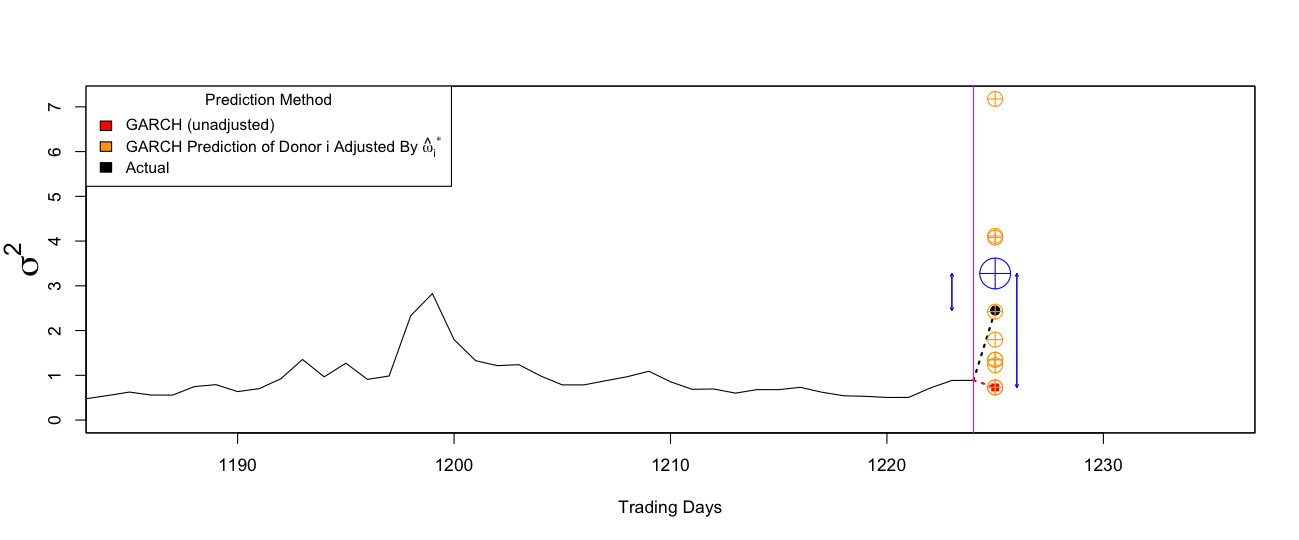
\includegraphics[width=\textwidth]{simulation_plots/motivating_piece_convex_combination.png}};
        % \draw[red,ultra thick,rounded corners] (7.5,5.3) rectangle (9.4,6.2);
        % \node[draw,text width=4.45cm] at (9.8,3.2) {$\textcolor{blue}{\hat\sigma^{2}_{adjusted} = \hat\sigma^{2}_{unadjusted} + \hat\omega^{*}}$ };
        % \node[draw,text width=2.62cm] at (14.8,2.8) {$\textcolor{blue}{\hat\omega^{*} = \sum^{n+1}_{i=2}\pi_{i}\hat\omega^{*}_{i}}$ };    
        
    \end{tikzpicture}
      \caption{The simulated time series experiences a volatility shock between trading days 1,656 and 1,657.  The GARCH prediction, in red, fails even to approach the volatility spike at $T^{*}+1$, as do several adjusted predictions, which are orange.  In contrast, the GARCH forecast adjusted by $\hat\omega^{*} = \sum^{n+1}_{i=2}\pi_{i}\hat\omega^{*}_{i} $, a convex combination of the estimated shocks in the donor pool, achieves directional correctness as well as a smaller absolute loss in its prediction.  The pink vertical line serves to indicate the adjustment of size $\hat\omega^{*}$ that allows the blue bullseye to approach more closely the ground truth.}    \label{fig:motivating_piece_convex_combination}
   
      \end{center}
    \end{figure}

We will suppose that a researcher has a multivariate time series data $\y_{i,t} = (y_{i,t}, \x_{i,t}$), $t = 1,$ $\ldots,  T_i$, $i = 1, \ldots, n+1$, where $r_{i,t}$ is scalar and $\x_{i,t}$ is a vector of covariates such that $\x_{i,t}|\mathcal{F}_{i,t-1}$ is deterministic and observed.  Suppose that the analyst is interested in forecasting $y_{1,t}$, the first time series in the collection, which we will denote \textit{the time series under study}.   We assume the following general data-generating process

  \begin{align}
    \mc{M}_1 \colon \begin{array}{l}
      y_{i,t} = F(\mathcal{F}_{i,t-1}) + \alpha_{i,t} + \epsilon_{i,t}\\[.2cm]\label{core_specification}
      \alpha_{i,t} = \x^{T}_{i,t}\lambda_{i,t} \\[.2cm]
     \x_{i,t}^{T} = (x^{1}_{i,t},...,x^{p}_{i,t},1)\\[.2cm] 
     \lambda_{i,t}^{T} = (\lambda^{1}_{t},...,\lambda^{p}_{t},u_{i,t}),\\[.2cm]
    \end{array}
    \end{align}
with time-varying and observable covariate vector $\x_{i,t}^{T}$, time-varying and unknown parameter vector
\begin{align*}
\lambda_{i,t} &\sim \mc{F}_{\lambda}\text{ with }  \E_{\mathcal{F}_{\lambda}}(\lambda) = \mu_{\lambda_{t}}, \mrm{Var}_{\mc{F}_{\lambda}}(\lambda) = \Sigma_{\lambda_{t}},\\
\end{align*}
and time-invariant error structure
  \begin{align*}
    \epsilon_{i,t} &\simiid \mc{F}_{\epsilon} \text{ with}  \; \E_{\mc{F}_{\epsilon}}(\epsilon) = 0, \mrm{Var}_{\mc{F}_{\epsilon}}(\epsilon)  = \sigma^{2}_{\epsilon},  \\
    %u_{i,t} & \simiid  \mc{F}_{u} \text{ with}  \; \mrm{Var}_{\mc{F}_{u}}(u) = \sigma^2_{u},\\
    % &\epsilon_{i,t} \indep u_{i,t},
    \end{align*}
where $F$ maps objects from the past into future objects of $y_{i,t}$, and $\epsilon_{i,t}$ uncorrelated across time and donors.  Note that the dot product $\alpha_{i,t} = \x^{T}_{i,t}\lambda_{i,t}$ includes the term $u_{i,t}$ that is not shared among donors.  It encodes the known possibility that the shocks will vary across donors both in ways that can predicted based on pre-shock covariates as well as in ways that cannot be predicted.  That the parameter vector is time-varying allows us to capture that most time points are without news shocks, but conditional upon information arriving between $T_{1}^{*}$ and $T_{1}^{*}+1$, we may know with near certainty that $\lambda_{1,T_{1}^{*}+h}$ will be nonzero in norm for some $h>0$.

The specification (\ref{core_specification}) above is sufficiently capacious as to include data-generating processes of the form 

\begin{align*} 
  y_{i,t} = \log{Y_{i,t}} = \log{a_{i,t}y_{i,t-k}e^{\alpha_{i,t}+\epsilon_{i,t}}} = \log{a_{i,t}} + \log{y_{i, t-k}} + \alpha_{i,t} + \epsilon_{i,t}
\end{align*}
with $k\geq1$ and $a_{i,t}, y_{i,t}$ supported on $\mathbb{R}^{+}$.  The term $\x^{T}_{i,t}\lambda_{i,t}$ will be deemed the $\textit{correction term}$, and the function

\begin{align*}
  \xi \colon \mathcal{F}_{2,T^{*}_{2}+h} \times \ldots \times \mathcal{F}_{n+1, T^{*}_{n+1}+h} &\to \mathcal{F}_{1,T^{*}_{1}+h}\\
\end{align*}
that estimates or predicts $\alpha_{1,T^{*}_{1}+h}$ will be deemed the \textit{correction function}.  The correction function maps observable, deterministic events and unobservable events into a space so that something might be learned about $\lambda_{i,t}$.  If $\x_{i,t}$ were not observable or not deterministic with respect to $\mathcal{F}_{t-1}$, then the correction term would represent an additional error term (not necessarily idiosyncratic).

We require that each time series $\y_{i,t}$ is subject to an observed news event following $T^*_i \leq T_{i} + 1$ and before witnessing $T^*_i+1$.  The reasons for this represent the heart and soul of the framework proposed.  We are not proposing a method to correct for unanticipated shocks that have been reflected in the observed data.  Instead, we are proposing a method to correct for shocks for which the qualitative kernel of information is known and the observed quantitative instantiation which is not yet known. 

So far we have reviewed a long and rich literature about model adjustment, and we have also introduced a data-generating process upon which the rest of this manuscript will be based.  We now proceed to introduce a particular framework of solutions to the circumstances assumed in Section \ref{Setting}.  What we are doing here is therefore not out of the ordinary but distinct in at least two ways: (1) we are incorporating outside information faster, and (2) we are proposing a principled, systematic way to do it that defies that curse of dimensionality.  If one wanted to forecast using linear models and high-dimensional information set, then some kind of method for reducing model complexity would be required.  We avoid that.

\section{SPC Forecasting Methodology and Correction Functions}

We now present two one-step-ahead forecasts for the time series under study. The first is the unadjusted forecast. The second is the adjusted forecast, which differs by the predicted correction term.  The forecasts are: 

\begin{align*}
  \text{Forecast 1: }& 
   \hat y_{unadjusted, T_{1}^{*}+1} = \hat\E[\mathcal{F}_{T_{1}^{*}}] \\
  \text{Forecast 2: }&
   \hat y_{adjusted,T_{1}^{*}+1} = \hat\E[\mathcal{F}_{T_{1}^{*}}] + \hat\alpha_{T^{*}_{1}+1} \text{ .}
\end{align*}
The problem of aggregating shocks or residuals begins with the data constraints.  Let us first introduce useful notation.  Let $\hat\alpha^{*}_{i,*}$ denote estimated correction term for donor $i$.   Taking the weights estimated correction terms as a given, we observe the tuple of information $(\{\hat\alpha_{i,*}\}^{n+1}_{i=2}, \mathcal{F}_{2,T^{*}_{2}}\times \ldots \times \mathcal{F}_{n+1,T^{*}_{n+1}}\})$ that is the extracted residuals as well as pre-shock information that may be important to aggregation.  
    
  One approach to aggregation comes from \cite{lin2021minimizing}, where weights belonging to the simplex, $\{\weight_{i}\}^{n+1}_{i=2} \in \Delta^{n-1}$, are chosen via a distance-based weighting procedure, resulting in the correction function 

\begin{align*} \label{adjustment}
	  \hat\alpha = \sum^{n+1}_{i=2}\weight_{i}\hat\alpha_{i,*},
\end{align*}
which is just one way among many to build a correction function.  Another interesting correction function can be found in \cite{foroni2022forecasting}.  For yet another example, consider a correction function that aggregates survey panel of forecasts by the Survey of Professional Forecasts \citep{croushore1993introducing}.  An obvious advantage of human forecasters is that they are able to integrate information revealed arbitrarily close to the scheduled release of the forecast, even if human forecaster's lack of systematicity or closed-form forecasts, for example, leads to non-optimal forecast performance in general.  By calculating forecast differences between the low-frequency information forecast, $\tau_{i,t}= \hat{y}_{unadjusted,t}-\hat{y}_{ i,t}$, we prepare ourselves for late-breaking events -- e.g. shocks -- for which we might want a correction function

\begin{align*}
\xi \colon \boldsymbol{\tau} &\to \mathcal{F}_{1, T^{*}_{1}} \\
\end{align*}
that weights the $i$-th forecaster according to that forecaster's past performance or according to the similarity of the forecaster's stated information set to the information available for the default forecasting model.

\section{Model Adjustment Using Similarity-Based Parameter Correction: A Global Overview}\label{global_overview}

In this section, we introduce and discuss a general framework for model adjustment that generalizes and is motivated by the circumstances laid out in Section \ref{Setting} by boiling down SPC to its essential five elements.  The essential elements of similarity-based parameter correction are

\begin{enumerate}
  \item \textbf{Object-to-predict}
  Most fundamentally, the method requires a random object (indexed over time, of course) that obeys a specification with additive errors, or, at the very least, a specification that can be transformed to have additive errors.  This requirement is suitably weak, so as to include models that are not linear or not linear in each of their parameters.  It also includes multidimensional objects as well as objects from non-Euclidean probability spaces, like some function spaces.  

Notice that we did not say \textit{parametric} specification.  The reason for this is that, given any forecast function $f$ from an information set $\mathcal{F}_{t}$, and given any appropriate loss function \textit{L}, we can define a residual $e_{t} = y_{t} \odot \hat{y_{t}}$, where $\odot$ is subtraction in the simple case of mean squared-error.  The residuals (or transformations of those residuals) of those $n$ models can be weighted as part of a correction function.  This fact is especially useful when the forecast function $f$ is nonparametric, black-box, or stochastic with respect to $\mathcal{F}_{t}$.

\item \textbf{Common Model Family on the Shocks} The method requires that residuals be governed by a model that is shared across all units.  This ensures that in the estimation of news shocks in the donor pool, the estimators will enjoy similar properties that will produce a good aggregated shock estimator.  This condition is satisfied by the parametric shock distributions found in \cite{lin2021minimizing,lundquist2024volatility}.

\item \textbf{Reliable and Shared Model-Fitting Procedure} There must exist a reliable model-fitting procedure for the $n+1$ units, one that will allow the assumption of a shared family for the residuals to be reflected in the residuals.  Here, reliable could mean any number of several things.  It means that the estimation procedure must produce a credible description of each data-generating process or a good prediction function, so as to aid in estimating residual in each unit.  `Reliable' may mean the estimators have low variance, and it may also mean that the estimation procedure is robust, to some degree, to misspecification bias.  However, in theory, the lack of these properties is not harmful to the method unless the lack of these properties harms the correction term's estimation.  When we use fixed effect estimation (under ordinary assumptions), we can construct confidence intervals for the fixed effect estimates, and then assuming independence, we can get confidence intervals for convex combinations of fixed effect estimates.

\item \textbf{Reliable Correction Term Estimation} Fourth, there must exist a reliable procedure for modeling and estimating the correction term in each unit.  Again, here we care about low variance as well as robustness to misspecification.  The very simplest correction term is the residual itself.  Alternatively, the correction term could be an inner product that depends upon external covariates, as is found in \cite{lin2021minimizing,lundquist2024volatility}.

This might not always be straightforward.  Some models like GARCH, for example, might deliver very noisy estimates for indicator variables that occur just once.

\item \textbf{Reliable Correction Function Estimation} There must exist a correction function (presumably based on the correction term) that maps data from the donor pool to the $\textit{predicted}$ correction term in the time series under study based on some notion of similarity.  In some cases, there may exist a posited DGP that the correction term estimates.  In other cases, there may be no posited DGP.  Similarly, if there exists a posited DGP for the correction term, it may depend upon data internal to the time series under study, or it may depend on external data, e.g. outside data could be aggregated (e.g. Nearest-Neighbor, arithmetic mean, kernel methods) to estimate the correction function.

\end{enumerate}

\section{Formal Properties and Model-Specific Considerations}\label{special_cases}

In this section, we discuss particular models for which our approach has been implemented as well as others for which it has yet to be implemented.  For those for which an implementation exists, we introduce the model in a more general light, while also commenting on the model-specific considerations.


\subsection{ARIMA}\label{ARIMA}
Recall the specification (\ref{core_specification}), which models a news shock as an affine function of covariates:

\begin{align*}
  &y_{i,t} = F(\mathcal{F}_{i,t-1}) + \alpha_{i,t} + \epsilon_{i,t}
\end{align*}
We begin our recounting of model-specific cases by recalling \cite{lin2021minimizing}, in which it was established that for a family of AR(1)-distributed scalar time series with a common shock distribution, forecast risk can be reduced via a similarity-based adjustment procedure.  An AR(p) is an easy model to work with, in part because it can be consistently estimated via OLS, and an AR(p) can approximate an ARMA(p,q) with arbitrarily-small error through via a truncation of an AR($\infty$) representation.  Setting aside the estimation method, consider a one-step-ahead for an AR(p) at time $t$ with an adjustment estimator, $\hat\alpha_{t}$:

\begin{align}
\hat{y}_{t} = f(\mathcal{F}_{t-1}) = \hat\mu + \sum^{p}_{i=1}\hat\rho_{i}y_{t-k} + \hat{\alpha}_{t}
\end{align}
which can be understood as an AR($p$) with time-varying coefficients.  The mean squared-error of the forecast above, i.e.

\begin{align}
  \E[(y_{t}-\hat{y}_{t})^{2}] &= \E[(y_{t} - \hat\mu + \sum^{p}_{k=1}\hat\rho_{k}y_{t-k} + \hat{\alpha}_{t})^{2}]\\
  &= \E[(\mu + \sum^{p}_{k=1}\rho_{k}y_{t-k} + \alpha_{t} + \epsilon_{t}  - (\hat\mu + \sum^{p}_{k=1}\hat\rho_{k}y_{t-k} + \hat{\alpha}_{t}))^{2}] \\
  &= \E[((\mu - \hat\mu) + \sum^{p}_{k=1}(\rho_{i}-\hat\rho_{k})y_{t-k} + (\alpha_{t} - \hat{\alpha}_{t}) + \epsilon_{t} )^{2}]\label{ARIMA_MSE_breakdown}
  \end{align}
admits of the typical bias-variance decomposition.  Taking $\mu = 0$, for simplicity, (\ref{ARIMA_MSE_breakdown}) becomes

\begin{align}
  &\E[(\sum^{p}_{k=1}(\rho_{k}-\hat\rho_{k})y_{t-k} + (\alpha_{t} - \hat{\alpha}_{t}) + \epsilon_{t} )^{2}]\\
  = &\text{Bias}^{2}[\sum^{p}_{k=1}(\rho_{k}-\hat\rho_{k})y_{t-k} + (\alpha_{t} - \hat{\alpha}_{t}) ] + \text{Var}[\sum^{p}_{k=1}(\rho_{k}-\hat\rho_{k})y_{t-k} + (\alpha_{t} - \hat{\alpha}_{t}) ] + \sigma^{2}_{\epsilon}\\
  = &\big[\E[\sum^{p}_{k=1}(\rho_{k}-\hat\rho_{k})y_{t-k} + (\alpha_{t} - \hat{\alpha}_{t}) ]\big]^{2} + \text{Var}[\sum^{p}_{k=1}(\rho_{k}-\hat\rho_{k})y_{t-k} + (\alpha_{t} - \hat{\alpha}_{t})]  + \sigma^{2}_{\epsilon}\\
  = &\big[\sum^{p}_{k=1}(\rho_{k}-\E[\hat\rho_{k}])y_{t-k} + (\alpha_{t} - \E[\hat{\alpha}_{t}]) \big]^{2} + \text{Var}[\sum^{p}_{k=1}(\rho_{k}-\hat\rho_{k})y_{t-k} + (\alpha_{t} - \hat{\alpha}_{t})]  + \sigma^{2}_{\epsilon}\\
  = &\big[\sum^{p}_{k=1}(\rho_{k}-\E[\hat\rho_{k}])y_{t-k} + (\alpha_{t} - \E[\hat{\alpha}_{t}]) \big]^{2} + \text{Var}[\sum^{p}_{k=1}\hat\rho_{k}y_{t-k} + \hat{\alpha}_{t}]  + \sigma^{2}_{\epsilon}\\
  = &\big[\sum^{p}_{k=1}(\rho_{k}-\E[\hat\rho_{k}])y_{t-k} + (\alpha_{t} - \E[\hat{\alpha}_{t}]) \big]^{2} + \text{Var}[\sum^{p}_{k=1}\hat\rho_{k}y_{t-k}] + \text{Var}[\hat{\alpha}_{t}]  + \sigma^{2}_{\epsilon}\tag{if shocks are uncorrelated with time series under study}\\
  = &\big[\sum^{p}_{k=1}(\rho_{k}-\E[\hat\rho_{k}])y_{t-k} + (\alpha_{t} - \E[\hat{\alpha}_{t}]) \big]^{2} + \text{Var}[\sum^{p}_{k=1}\hat\rho_{k}y_{t-k}] + \sum_{i=2}^{n+1}\pi_{i}^{2}\text{Var}[\hat\alpha_{i,t}] + 2\sum_{i\neq j}\pi_{i}\pi_{j}\text{Cov}[\hat\alpha_{i,t},\hat\alpha_{j,t}]  + \sigma^{2}_{\epsilon}
\end{align}

Assume we have no control over the accuracy of the estimates $\hat\rho_{k}$ nor any control over the estimates $\{\hat\alpha_{i,t}\}_{i=2}^{n=1}$.  Then our only control over the MSE comes from our choice of the $\hat\alpha_{t}$, over which our only control comes from the weight vector $\vec{\pi}$, so long as it is not unique.  If we insist that $\hat\alpha$ be an unbiased predictor, then the MSE is minimized by vector $\vec{\pi}$ --- again, not necessarily unique --- that will generally be sparse, so as to zero-out the covariance terms.  All of this is to say that control of the MSE may require tight control of the variance in the prediction function, which in turn will gesture in the direction of a sparse $\hat\alpha_{t}$ and sparse estimation of the autoregressive structure.


%https://tex.stackexchange.com/questions/174317/creating-a-labeled-tetrahedron-with-tikzpicture
\begin{figure}
\centering
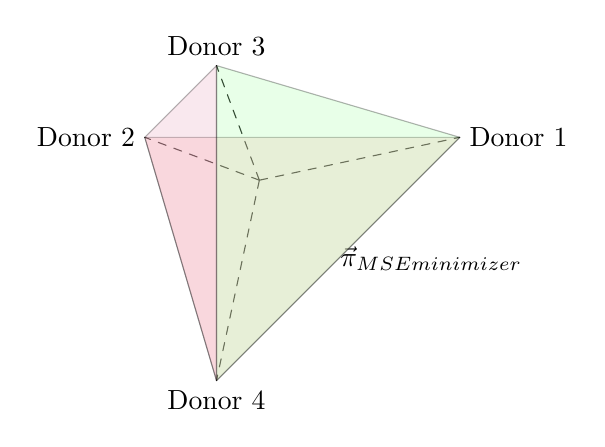
\begin{tikzpicture}[line join = round, line cap = round]
\pgfmathsetmacro{\factor}{1/sqrt(2)};
\coordinate [label=right:Donor 1] (1) at (2,0,-2*\factor);
\coordinate [label=left:Donor 2] (2) at (-2,0,-2*\factor);
\coordinate [label=above:Donor 3] (3) at (0,2,2*\factor);
\coordinate [label=below:Donor 4] (4) at (0,-2,2*\factor);
\coordinate [label=below:$\vec{\pi}_{MSE minimizer}$] (5) at (2.1,-.8,-.3*\factor);


% \draw[->] (0,0) -- (3,0,0) node[right] {$x$};
% \draw[->] (0,0) -- (0,3,0) node[above] {$y$};
% \draw[->] (0,0) -- (0,0,3) node[below left] {$z$};
\foreach \i in {1,2,3,4}
    \draw[dashed] (0,0)--(\i);
\draw[-, fill=red!30, opacity=.3] (1)--(4)--(2)--cycle;
\draw[-, fill=green!30, opacity=.3] (1) --(4)--(3)--cycle;
\draw[-, fill=purple!30, opacity=.3] (2)--(4)--(3)--cycle;
\end{tikzpicture}
\caption{The 3-Simplex, $\Delta^{3}$, where hypothetical minimizer is a convex combination of Donors 1 and 4.}
\end{figure}


\begin{prop}\label{ARIMA_param_consistency}
Let $2\leq i \leq n+1$.  The tuple of estimators ($\hat\rho_{1},...,\hat\rho_{p}, \hat\alpha_{i,t}$) is consistent as $t \rightarrow \infty$.
\end{prop}

\begin{prop}\label{ARIMA_conv_distribution}
  Let $\{\hat y_{1,T_{1}^{*}+r}\}^{h}_{r=1}$ denote the vector of adjusted predictions (adjusted through $h$ steps ahead) in the time series under study.  $\{\hat y_{1,T_{1}^{*}+r}\}^{h}_{r=1} \xrightarrow{d} \{ y_{1,T_{1}^{*}+r}\}^{h}_{r=1}$.
  \end{prop}

When forecasting financial time series using the method above, the question of prices versus returns (or in the language of economics or engineering, levels versus flows) is relevant.  Consider, for example, the persistence of a shock.  A shock to an asset's return series at time $t$ implies a persistent shock to the asset's price series at time $t$ and beyond, as one can verify by inverting the discrete-differencing operation on a time series.  However, if one forecasts the price series of the asset directly, that persistence beyond the first instantiation of the shock must be modeled explicitly.  This suggests interesting opportunities in the analysis and forecasting of shock persistence for situations in which level-forecasting is appropriate, e.g. for stationary time series.

We now turn to the limitations of linear time series model class like ARIMA.  The first is that linearity is a nontrivial restriction, and for the purpose of modeling financial time series, applications of SPC to TAR and SETAR would be welcome.  Additionally, the efficient market hypotheses implies that market prices reflect all publicly-available information, which in turn implies that ARIMA models should be of no predictive value for market returns.  This critique, in a technical sense, alleges that market returns are random walks centered at zero, and for that reason, the coefficients of an ARMA approximation to a financial return series are uniformly zero, and that any incipient deviation from that equilibrium would not go unnoticed by market participants, who would exploit those deviations and push the coefficients back to zero, leaving only idiosyncratic noise.  Such concerns about forecasting in markets with heavy feedback loops motivates our next section.
\subsection{GARCH}
The methods of \cite{lin2021minimizing} are adapted in \cite{lundquist2024volatility} to forecast volatility.  This is in response to concerns we raised above about the usefulness of ARIMA models for forecasting financial returns as well as concerns about heteroskedasticity.  Financial time series are known to have both time-varying volatility as well as  volatility that \textit{clusters}, i.e. with volatile trading periods that bunch together.  A GARCH model, under weak conditions, is an ARMA model on the squared residuals of a time series, and empirical evidence strongly suggests that those ARMA (i.e. GARCH) coefficients are not zero, in general.  The predictability of either those squared returns or the predictability of $\sigma_{t}^{2}$ (in this context, the two tasks reduce to one) is bounded, however, by a function of the kurtosis of a GARCH process \citep{francq2019garch}.  That the GARCH model accommodates excess kurtosis in both the unconditional and conditional returns of a financial asset is a feature of the model, and perhaps for that reason, it has been noted that GARCH models do a much better job at modeling the evolution of volatility (a descriptive or inferential objective) as opposed to forecasting volatility.

In this way, \cite{lundquist2024volatility} bridged a gap between the descriptive and predictive roles of GARCH.  Fixed effects (correction terms) are estimated in the donor pool, and those fixed effects are aggregated via corrected function.  A forecast adjustment is then made in the time series under study.

\subsection{HAR}

The Heterogeneous Autoregressive (HAR) model for realized volatility \citep{corsi2009simple}  uses ordinary least-squares (OLS), WLS, or some other appropriate linear model to fit a predictive regression model.  It explores the influence of previous volatility on current volatility, of course, but uses a specification motivated by theory: that a heterogeneous collection of market participants interacts at different frequencies.  Therefore, the volatility can be well-modeled as a linear combination of the average volatility over the previous day, previous week, and previous month (usually taken to be 22 days).  Formally, HAR assumes that the log price of an asset is a governed by a diffusion process (a model beyond our scope herein), and HAR estimates

\begin{align*}
RV_{t} = \beta_{0} + \beta_{\text{1-day}}RV_{t-1} + \beta_{\text{5-day}}\overline{\{RV_{t-1},...,RV_{t-5}\}}+\beta_{\text{22-day}}\overline{\{RV_{t-1},...,RV_{t-22}\}} + \epsilon_{t}
\end{align*}
Recently, \cite{bodilsen2023exploiting} find that overnight news improves the predictive ability of HAR regressions with a logarithmic transformation on the realized volatility estimate.  The authors distinguish between earnings-related and non-earnings-related news occurring after hours, finding that predictive performance is improved for one-day-ahead forecasts but no more.

We should note that the regressions under discussion here are predictive regressions, with no suggestion that the model is fundamentally driven by the linear specification that is estimated.  However, if it were, we would especially desire answers to the following

\begin{enumerate}
  \item Are the relevance and novelty filters used by \cite{bodilsen2023exploiting} appropriate, and does it represent a qualitative decision?  Does it represent an instance of similarity-based matching?
  \item Could we relax the requirement on the relevance score and instead let a numerical algorithm determine which stories and relevant and how relevant?
  \item Could we relax the requirement on the novelty score?
  \item Bias-variance tradeoff: are we able to reduce the bias or the variance or both via the method of \cite{bodilsen2023exploiting}?
  \item What is the `frontier' that separates using a similarity-based approach like SPC as opposed to an approach using count variables?
  \item Can we confirm the theory that count variable approaches reduce variance while, as is well-established, SPC reduces bias?
  \item Does SPC do better when the shock is a nonlinear function of the covariates compared to a method that uses regression terms for each covariate?  Does SPC do better under those circumstances compared to count variable-based approaches?
  \item What are advantages and disadvantages of using counts versus indicator variables versus alternatives?
  \item  What DGP on overnight firm-specific news would most justify the approach in \cite{bodilsen2023exploiting}?
  \item Is earning-related and non-earnings-related the appropriate disaggregation to use?
  \item Is it appropriate to use counts at each time point, or would indicator variables be superior, or rather, under what conditions would indicator variables be superior?

\end{enumerate}

\subsubsection{A Real Data Application of Shock-Adjusted HAR Forecasting}

\begin{figure}[h!]
  \begin{center}
    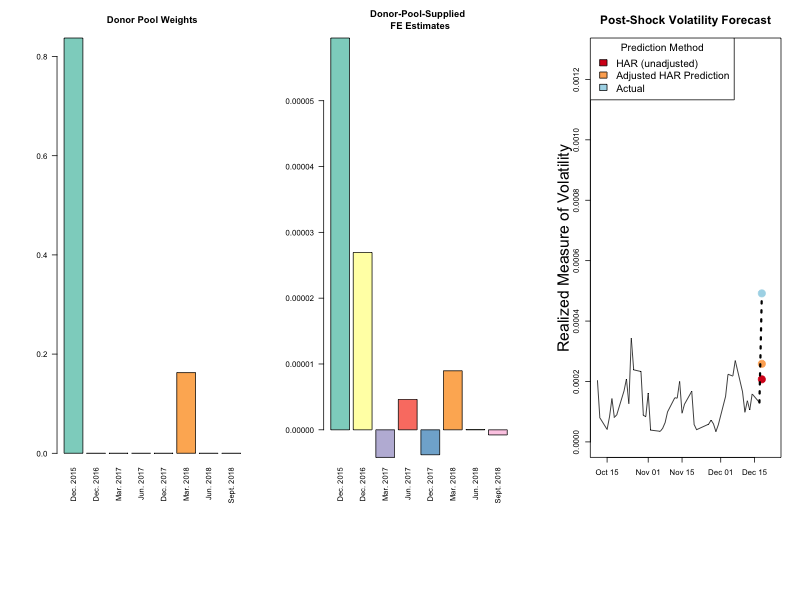
\includegraphics[scale=.4]{real_data_output_plots/savetime_SatJun151644072024__^VIX-^IRX-^XAU_^VIX_2018-12-18-2015-12-15-2016-12-13-2017-03-14-2017-06-13-2017-12-12-2018-03-20-2018-06-12-2018-09-25.png}
    \caption{Over the course of the 2010s, the US FOMC began a rate-hiking cycle.  Left pane: weights of the donor pool of FOMC meetings; right-pane: fixed effect estimates; right pane: the unadjusted forecast, adjusted forecast, and actual forecast}
    \label{fig:six_plots}
    \end{center}
  \end{figure}

% \subsection{VAR}
% Many time series, especially macroeconomic time series, naturally arise as constituents of groups of dependent variables that interact across time.
\subsection{LSTM/GRU}

\cite{hendry2004pooling} discuss that intercept correction can improve forecasts under structural breaks as well as under ``deterministic misspecification'', by which they mean misspecification not caused by stochastic events like location shifts.  The same two justifications exist for SPC: we can use SPC when we know there to be a structural break, and we can also use it when we know our model is wrong but lack knowledgde of precisely how it is wrong, and yet nevertheless wish to correct a parameter for some critical forecasting task.

One reason we may believe that our forecasting model is misspecified is that our forecast function is non-parametric, and hence the deterministic or stochastic mechanism through which we produce our forecasts does not involve parametric assumptions.  Here we demonstrate the tremendous capaciousness of SPC by applying it to predictions generated by a pair of non-parametric forecasting functions, Long Short Term Memory and GRU.  We will re-examine an application found in \cite{lin2021minimizing}.

We borrow code from \cite{Brownlee_2022}

\begin{itemize}
  % \item \href{https://www.r-bloggers.com/2021/04/lstm-network-in-r/#google_vignette}{a}
  % \item \href{https://sharmasaravanan.medium.com/an-implementation-guide-for-lstm-in-r-2347e4118a2c}{b}
  % \item \href{https://search.r-project.org/CRAN/refmans/TSdeeplearning/html/GRU_ts.html}{c}
  % \item \href{https://medium.com/codex/time-series-prediction-using-lstm-in-python-19b1187f580f#:~:text=In%20conclusion%2C%20LSTM%20models%20are,in%20your%20data%20science%20toolkit.}{d}
  \item \href{https://machinelearningmastery.com/time-series-prediction-lstm-recurrent-neural-networks-python-keras/}{LSTM in Python}
\end{itemize}

\subsection{``Exponential Breaks"}
In \cite{castle2011forecasting}, the authors discuss intercept shifts that decay deterministically.  Those shifts are parameterized by a scalar $\lambda$ and a decay rate $\psi$.  We adapt their model for our own purposes:

\begin{align}
y_{i,t} = \alpha_{i} + \lambda[1 - e^{-\psi[t-T_{i}^{*}+1]}]\textbf{1}_{t\geq T_{i}^{*}+1} + \epsilon_{i,t}, \epsilon_{i,t} \simiid [0,\sigma^{2}] \text{ .}\label{decay_model}
\end{align}
This poses a novel case for our method, in that the model is parametric and yet without estimability of all shock parameters, aggregation may not be straightforward or easy.  Consider, for any $i$, $2 \leq i \leq n+1$, the estimates $\hat\alpha_{i,OLS}$  obtained via regression on the first $T_{i}^{*}+1$ points as well as $\hat\lambda_{OLS}$ obtained by estimating a fixed effect at $t=T_{i}^{*}+1$.  Consider also a subsequent estimator, an estimator for $\psi$, that is derivable from inverting the model specification and plugging-in the estimates  $\hat\alpha_{i,OLS},\hat\lambda_{OLS}$:

\begin{align}
\hat\psi_{i,plugin} = \frac{1}{T_{i}-(T_{i}^{*}+2)}\sum^{T_{i}}_{t\geq T_{i}^{*}+2}-log{\big[-\big(\frac{y_{i,t}-\hat\alpha_{i}}{\hat\lambda} -1\big)\big]} / [t-T_{i}^{*}+1]\text{ .}\label{plugin}
\end{align}
(\ref{plugin}) is, to put it lightly, a complicated estimator with potentially dubious properties.  To begin, (\ref{plugin}) is defined only when the term inside the logarithm is positive for each $t\geq T^{*}_{i}+2$.  We could get around this by dropping any summands for which that term is nonpositive and instead calculate an average over only the remaining subset of summands.  Additionally, variance estimates for $\hat\psi_{i,plugin}$ may require resampling methods or the delta method.  Estimation error from $\hat\alpha$ and $\hat\lambda$ would naturally propagate to $\hat\psi_{i,plugin}$, and the expected estimation error would depend upon the size of the pre-shock sample.

\cite{castle2011forecasting} report that MSFE is lower by using intercept correction instead of non-linear methods to estimate $\psi$.

Now consider a practitioner in need of a conditional forecast for $T_{1}^{*}+h, h\geq 1$.  Could aggregating the prediction residuals $r_{i,T_{i}^{*}+h} = y_{T_{i}^{*}+h}-\hat y_{i, T_{i}^{*}+h}, h\geq 1$ lead us to a superior predictions in the time series under study?\\

\textbf{Consider also these complicating scenarios}
\begin{enumerate}
  \item We can estimate $\lambda$ using a cross-sectional regression, and that may be better estimator than doing it one-by-one in each donor.
  \item Here we have taken $\lambda$ to be fixed and shared across donors.  If $\lambda$ is a random, however, then estimating it becomes harder.
\end{enumerate}

\subsection{The Method of Multiple Shocks, Dual Shocks, and Shock-Partitioning}

Sometimes, we might have reason to believe that a forecast requires adjustment due to not one but multiple shocks.  \cite{lin2021minimizing} explored a ``dual'' shock in their analysis of oil company equity price shocks due to the March 2020 COVID lockdowns.  \\

Method 1: for each source of the $k$ shocks, assemble $n_{j}$ donors and $p_{j}$ covariates, with $j=2,...,n_{j}+1$, compute weights $\{\pi_{i,j}\}^{n_{j}+1}_{i=2}$.  With these $k$ weight sets, a set of $k$ aggregated shock estimators can be constructed and averaged (or aggregated in some other way).

Method 2: the $k$ shocks can be represented using one application of distance-based weighting, with the vector $\delta$ and the vector $\x_{i,T^{*}_{i}+1}$ can encode a partition of shocks by using zeros in appropriate entries.

\section{Discussion}

The forecast horizon --- does it matter?  If so, how so?  \cite{lin2021minimizing} has a one-period horizon.  \cite{clements1998forecasting}{p. 203} discuss how long to keep the forecast adjustment in place.  For a corrected ``slope parameter'', the effect of $h$ is not so clear.\\

\subsection{Shock propagation and estimation accuracy}
Consider \cite{lundquist2024volatility}, in which a real world example shows how volatility can be forecasted following surprising election outcomes.  There, the estimation of fixed effects is done around elections in a donor pool.  That means that for each past election or poll, etcetera, the method must accurately estimate the surprise-induced volatility boost.  That means picking a window around such an effect.\\

\textbf{proposals}
\begin{enumerate}
  \item For a given data-generating process, simulate the accuracy and variability of shock estimates using post-shock measurement periods of difference lengths.
  \item Develop formal results to quantify (estimate, bound, etc) the risk of using different post-estimation measurement lengths.  This matters because it might be that a donor has experienced a shock in the last $m$ days, and if $m$ is too small, using that donor may be risky.
\end{enumerate}
    

\subsection{Aggregating residuals as opposed to aggregating fixed effect estimates?}

Cases:
\begin{enumerate}
  \item Fixed effect is estimated with accuracy 
  \item Fixed effect is estimated with considerable noise.  Hence, the idiosyncratic error is estimated with considerable noise.
  \item idiosyncratic error large
  \item idiosyncratic error small
\end{enumerate}  

\section{Extensions}\label{Extensions}

\begin{itemize}
  \item Forecast for series besides the mean or conditional mean \textcolor{red}{If you have a family of models estimated used a Gaussian loss function, and the post-shock residuals are not conditionally Gaussian (e.g. they could be conditionally Cauchy), then why even start with the default forecasting function?  Why not throw it out entirely?  If only the distribution of the innovations changes, then would that even matter for a forecast that is purely concerned with the conditional mean?} Yet another potential motivation springs from the way we evaluate model performance.  In \cite{clements2005evaluating}, the authors discuss six dichotomies regarding forecast evaluation as a way of advising caution about simplistic notions of performance evaluation.  These ideas matter for the current manuscript for at least one reason.  We must entertain the possibility that breaks in the DGP will invalidate the standard forecast evaluation framework under which we had been working.  If, for example, we have a family of models estimated used a Gaussian loss function, and the post-shock residuals are not conditionally Gaussian (e.g. they could be conditionally Cauchy), then why even start with the default forecasting function?  Why not throw it out entirely?  If only the distribution of the innovations changes, then would that even matter for a forecast that is purely concerned with the conditional mean?
  \item Bias-variance decomposition for ARIMA, as introduced in (\ref{ARIMA})
  \item Shrinkage estimation of autoregressive structure on all donors, then use our method
  \item TAR
  \item SETAR
  \item Function forecasts
  \item Binary Outcome Forecasts
  \item Density Forecasts
  \item Quantile Forecasts
\end{itemize}

\subsection{Forecast Combination}
what we are talking about here is not forecast combination, but there may be, nevertheless, a role for forecast combination: combining the forecasts generated by small differences in covariate and/or donor choice, as is done in \cite{lundquist2024volatility}. \\

Consider the leave-one-out method used on pairs of donors and covariates in \cite{lundquist2024volatility}.  By averaging over $(n+1)\cdot (p+1)$ predictions, we average over $(n+1) \cdot (p + 1)$ convex combinations (where, when a donor is ommitted, its weight can be imputed as zero).

\subsection{Limitations}\label{Limitations}

\subsubsection{How important is a shared DGP?}
In particular, can we relax this assumption and proceed with weaker assumptions on the donors and time series under study?

\subsubsection{The assumption of a shared family can be relaxed in certain circumstances.  For example, if a certain donor is not like the time series under study with respect to the covariates, then the lack of a shared family will not matter much.}


\textbf{In Scope}
\begin{itemize}
  \item Introduce an existing diffuse set of approaches to adjusting forecasts (\ref{Introduction})
  \item Explain when/how similarity can help us forecast. \ref{outside_info}
  \item distinguish the method from various tools that inspired it (\ref{Introduction})
  \item show a few special cases, both examples and formal results (\ref{special_cases})
  \item discuss limitations of the method (\ref{Limitations})
  \item propose extensions (\ref{Extensions})
\end{itemize}
\textbf{Beyond Scope (but mentioned briefly)}
\begin{itemize}
  \item Wade too deeply into distance-based weighting details.  State that it's simply one way to do it.  Allude to \cite{lin2021minimizing,lundquist2024volatility}.
  \item wade too deeply into any of the special cases
  \item Tackle non-scalar random quantities (density forecasts, etc)
  \item Forecast combination
\end{itemize}

\section{Supplement}


\subsection{Formal Results}

\begin{proof-of-proposition}[\ref{ARIMA_param_consistency}]
  We claim
  \begin{align}
  \mathbb{E}[ \sigma^{2} ]
  \end{align}
  
  \end{proof-of-proposition}

  \begin{proof-of-proposition}[\ref{ARIMA_conv_distribution}]
    We claim
    \begin{align}
    \mathbb{E}[ \sigma^{2} ]
    \end{align}
    
    \end{proof-of-proposition}
  
\clearpage
\bibliographystyle{plainnat}
\bibliography{unifying.bib}
 
\end{document}